\documentclass{beamer}
\usepackage{hyperref}
\usepackage{bookmark}
\usepackage{amsmath}
\usepackage[T1]{fontenc}
\usefonttheme[onlymath]{serif}
\usepackage[spanish,provide=*]{babel}
% Cargar apacite después de babel para citas autor-año correctas

% other packages
\usepackage{latexsym,amsmath,xcolor,multicol,booktabs,calligra, tcolorbox}
\usepackage{graphicx,listings,stackengine}
% Manejo robusto de nombres de archivo con espacios y rutas de imágenes
\usepackage{grffile}
%\graphicspath{{pic/}}



\author{Dylan Jara}
\title[Modelamiento de Lahares mediante PINNs]{Modelamiento de Lahares mediante Redes Neuronales Informadas por la Física (PINNs): Aplicación 
al evento eruptivo de 2015 del volcán Villarica, Chile}
\subtitle{}
\institute{
    Departamento de Matemática y Ciencia de la Computación, Universidad de Santiago de Chile
}
\date{\today}
\usepackage{./Ritsumeikan}

% defs
\def\cmd#1{\texttt{\color{red}\footnotesize $\backslash$#1}}
\def\env#1{\texttt{\color{blue}\footnotesize #1}}
\definecolor{deepblue}{rgb}{0,0,0.5}
\definecolor{ccnuMainColor}{RGB}{57,64,73}
\definecolor{deepgreen}{rgb}{0,0.5,0}
\definecolor{halfgray}{gray}{0.55}

\lstset{
    basicstyle=\ttfamily\small,
    keywordstyle=\bfseries\color{deepblue},
    emphstyle=\ttfamily\color{ccnuMainColor},    % Custom highlighting style
    stringstyle=\color{deepgreen},
    numbers=left,
    numberstyle=\small\color{halfgray},
    rulesepcolor=\color{red!20!green!20!blue!20},
    frame=shadowbox,
}

\begin{document}

\begin{frame}
    \titlepage
    \vspace*{-0.6cm}
    \begin{figure}
        \begin{center}
                % Ajuste de tamaño más visible y uso de \graphicspath
                
\includegraphics[keepaspectratio, width=0.25\textwidth]{./Pics/Usach S1.png}

        \end{center}
    \end{figure}
\end{frame}

% Restaurar la tabla de contenidos y corregir el problema de 'Referencias32'
\begin{frame}
    \tableofcontents[sectionstyle=show, subsectionstyle=show/shaded/hide]
\end{frame}

%//////////////////////////////////////////////////////%
\section{Introducción}
\subsection{Lahares}
\begin{frame}{Qué son los lahares?}
    \begin{itemize}
        \item<1-> Flujos de sedimentos volcánicos que se originan en volcanes potencialmente activos se llaman lahares \textbf{\cite{Vallance2024}}.
        \item<2-> Los lahares son mezclas de agua, ceniza volcánica, tefra, fragmentos de roca y bloques de hielo que pueden fluir como concreto húmedo. 
        \item<3-> El término proviene de la palabra indonesia para estos destructivos flujos de lodo que causan tanto daños materiales como pérdida de vidas. \cite{porfido2020new,ortiz1996riesgo}
    \end{itemize}
\end{frame}

\begin{frame}
    \begin{figure}
        \centering
        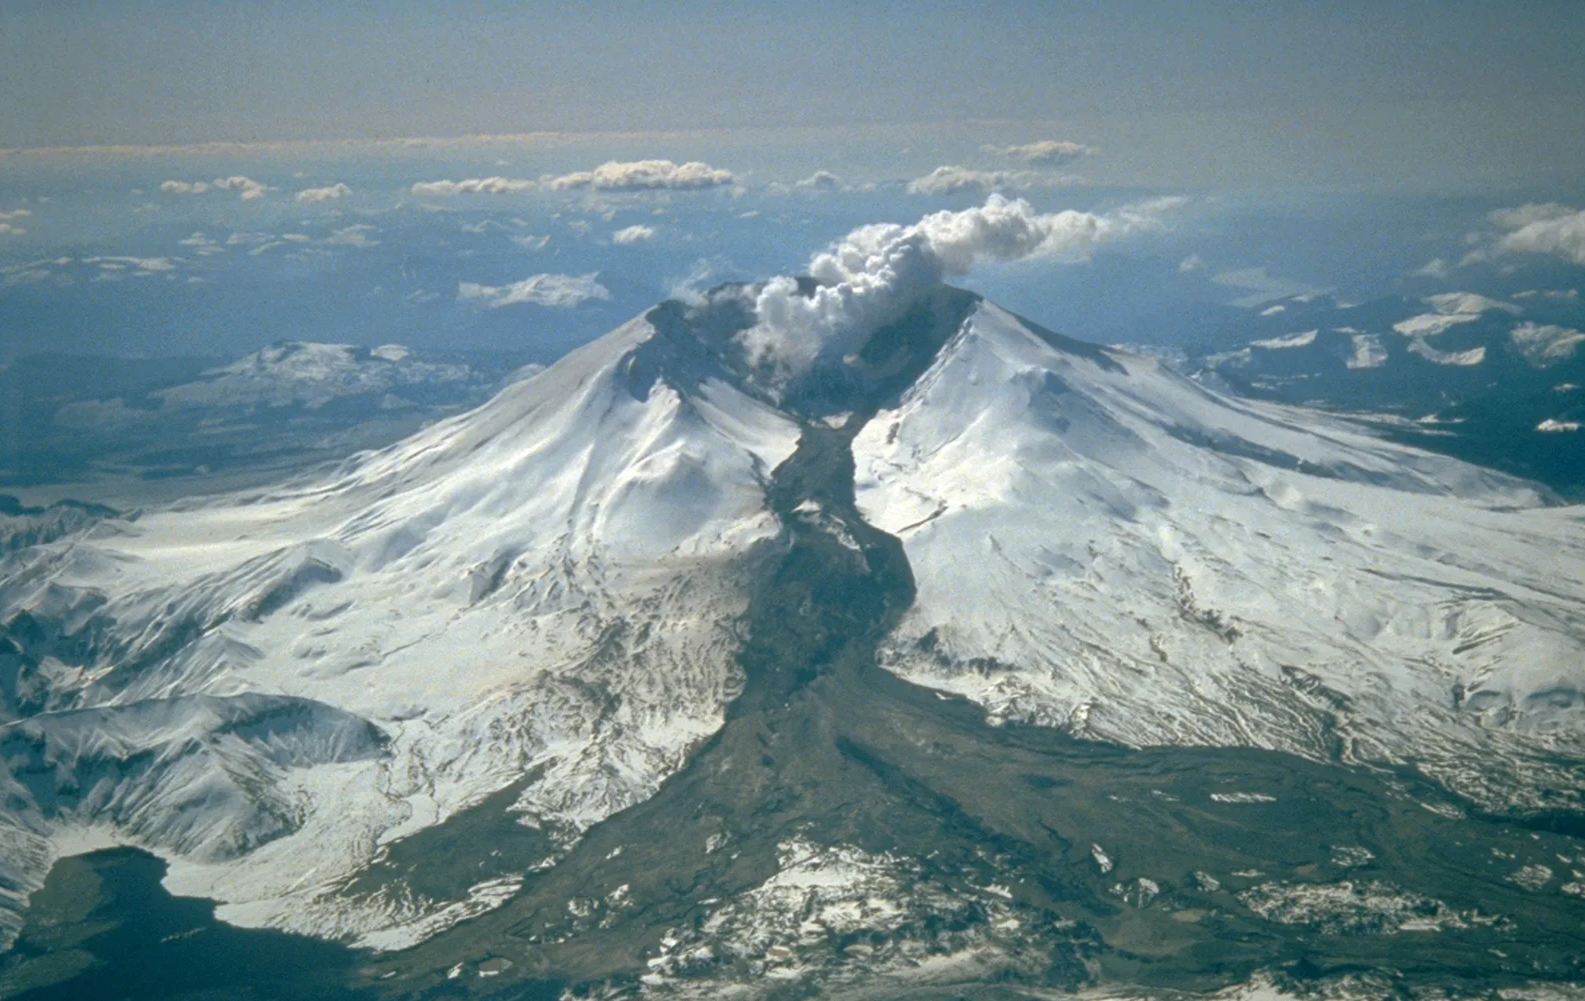
\includegraphics[width=10cm,height=6cm]{.//Pics//lahar.png}
        \caption{Lahar (dark deposit on snow) on Mount Saint Helens after the March 19, 1982, eruption.\cite{article}}
    \end{figure}
\end{frame}

\subsection{Physics-Informed Neural Networks (PINNs)}
\begin{frame}{Que son las PINNs?}
\begin{itemize}
    \item Las redes neuronales basadas en la física son redes neuronales entrenadas para resolver tareas de aprendizaje supervisado respetando
    cualquier ley física dada descrita por ecuaciones diferenciales parciales no lineales generales. \cite{RAISSI2019686}
    \item Estas redes neuronales están obligadas a respetar cualquier simetría, invariancia o principio de conservación que se derive de
    las leyes físicas que rigen los datos observados, tal como se modelan mediante ecuaciones diferenciales parciales no lineales y dependientes del tiempo.
\end{itemize}
\end{frame}

\begin{frame}{PDEs y residuos en la PINN}
\begin{itemize}
    \item $\mathcal{L} = \mathcal{L}_{data} + \lambda \mathcal{L}_{physics}$, donde $\mathcal{L}_{data}$ mide el error en los datos y $\mathcal{L}_{physics}$ mide el incumplimiento de las PDEs.
\end{itemize}
\end{frame}


\section{Objetivos}
\begin{frame}
    
    \begin{block}{Objetivo general}
        Desarrollar un modelo de lahares basado en Redes Neuronales Informadas por la Física (PINNs), aplicado al evento eruptivo de 2015 del volcán Villarica, Chile, incorporando ecuaciones acopladas de flujo somero, concentración sólida y presión de poros.
    \end{block}
    
    \begin{block}{Objetivos específicos}
        \begin{enumerate}
            \item Formular un sistema acoplado de Ecuaciones Diferenciales Parciales (PDEs) que modelen la morfodinámica de un lahar, incorporando conservación de masa, momento, concentración sólida y presión de poros.
            \item Construir una Red Neuronal Informada por la Física, basada en un sistema de ecuaciones diferenciales y parámetros geológicos, con la finalidad de predecir el comportamiento real de un flujo de sedimento. 
        \end{enumerate}
    \end{block}
\end{frame}

\begin{frame}
    \begin{block}{Objetivos específicos}
        \begin{enumerate}
            \item Diagnosticar patologías de desvanecimiento y decaimiento de los gradientes e incorporar técnicas de estabilización y optimización avanzadas para mejorar la convergencia del modelo.
            \item Predecir la morfodinámica de manera realista y acorde a la física para exportar un mapa de peligro volcánico que entregue datos de evacuación según el riesgo calculado por la red neuronal.
        \end{enumerate}
    \end{block}
\end{frame}


%/////////////////////////////////////////////%
\section{Estado del Arte}
\begin{frame}{Métodos numéricos actuales para predicción}
\begin{itemize}
    \item LAHARZ es un modelo computacional que utiliza descripciones estadísticas de áreas inundadas por eventos pasados de flujo masivo 
    para pronosticar áreas que probablemente serán inundadas por eventos hipotéticos futuros. \cite{schilling2008using}
    \item D-Claw es una biblioteca de software para la simulación de flujos granulares densos sobre topografía espacialmente variable. \cite{george2025d}
    \item LaharFlow es un software de dinámica de lahares, diseñado en la Universidad de Bristol, que modela el flujo de lahar como una mezcla de agua y granos sólidos, basado en tres principios
    de conservación. Estos son conservación de la masa, momentum y transporte de material sólido \cite{woodhouseshallow}
\end{itemize}

\end{frame}


%/////////////////////////////////////////////%
\section{Variables y parámetros}
\begin{frame}{Variables y parámetros}
\begin{itemize}
    \item $h(x, y, z, t)$: espesor de la mezcla $(m)$,
    \item $u(x, y, z, t), v(x, y, z, t)$: velocidades promediadas en profundidad $(m/s)$,
    \item $C(x, y, z, t)$: concentración volumétrica de sólidos $(\text{adimensional}, 0 \leq C \leq 1)$,
    \item $z_b(x, y, z, t)$: elevación del lecho $(m)$.
\end{itemize}
\end{frame}


\section{Sistema acoplado de PDEs}
\begin{frame}{Conservacion de Masa y Momentum}
    Conservacion de masa con fuente de masa: 
    \begin{align}
    {\partial h \over \partial t} + \nabla \cdot (h \vec{u}) = S_h(x,y,t), && u=(u,v)
    \end{align}
    Conservacion de momentum 2D con friccion basal modulada:
    \begin{align}
    {{\partial u} \over{\partial t}}+u{{\partial u} \over{\partial x}}+v{{\partial u} \over{\partial y}}+g{{\partial H} \over{\partial x}}+{{\tau_{bx}} \over{\rho_mh}} = 0 \\
    {{\partial v} \over{\partial t}}+u{{\partial v} \over{\partial x}}+v{{\partial v} \over{\partial y}}+g{{\partial H} \over{\partial y}}+{{\tau_{by}} \over{\rho_mh}} = 0
    \end{align}
    Donde la tension basal es parametrizada como 
    \begin{align}
    \tau_{b} = \tau_{b}\frac{u}{\|u\|+\epsilon},&&\tau_{b}=\mu_{eff}(C,p)\rho_mgh \cos\theta
    \end{align}
\end{frame}

\begin{frame}{Conservación de Momentum}
    La pendiente se aproxima por:
    \begin{align}
        \cos\theta\approx \frac{1}{\sqrt{1+\|\nabla z_b\|^2}}
    \end{align}
    Un modelo reducido pero físicamente interpretable para fricción efectiva:
    \begin{align}
        \mu_{eff}(C,p) = \mu_0(1+\alpha_C(C-C_0))\exp(-\alpha \frac{p}{\rho_mgh+p_{ref}})
    \end{align}
    donde C0 es una concentración de referencia y pref estabiliza la razón. Este término representa: (i) mayor fricción con mayor carga sólida, y 
    (ii) menor fricción efectiva cuando el exceso de presión de poros es alto (disminuye el esfuerzo efectivo).

\end{frame}

\begin{frame}{Ecuación de transporte de solidos (Advección-difusión)}
    Ecuación advección–difusión con término de relajación hacia un equilibrio
    \begin{align}
    {\partial C \over \partial t} + u\cdot \nabla C = \nabla \cdot (k_C\nabla C) + \frac{C_{eq}(x,y)-C}{\tau_C}
    \end{align}
    En prototipo sintético se puede fijar $\tau C \rightarrow \infty$ (sin relajación) o definir $C_{eq}$ como mayor en cauces y menor en planicies.
\end{frame}


\begin{frame}{Evolución de presión de poros}
    \begin{figure}
    \centering
    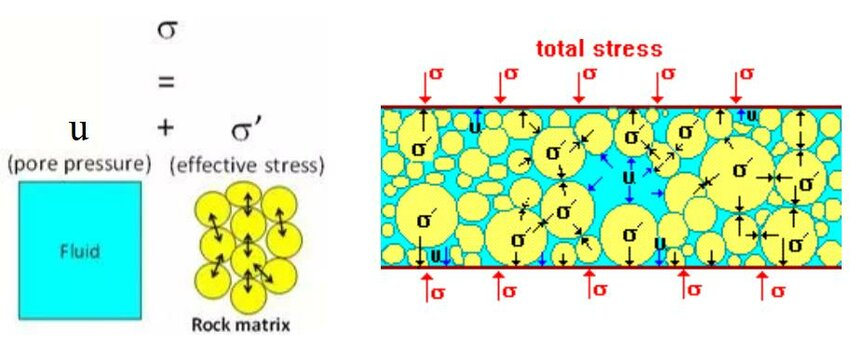
\includegraphics[width=10cm,height=6cm,keepaspectratio]{.//Pics//porepressure.png}
    \caption{Diagram illustrating the effective stress principle in a saturated cohesionless soil \cite{phdthesis}}
    \end{figure}
\end{frame}
\begin{frame}{Evolución de presión de poros}
    Se usa una ecuación de advección con relajación:
    \begin{align}
    {\partial p \over \partial t} + u\cdot \nabla p = \frac{p_{eq}(h,C,\|u\|)-p}{\tau_p}
    \end{align}
    Un ejemplo simple para equilibrio de presión:
    \begin{align}
        p_{eq}=\chi_p\rho_m gh\phi(C)\frac{\|u\|}{\|u\|+u_*}, && \phi(C)=\frac{C}{C+C_*}
    \end{align}
    que aumenta con espesor y con concentración, y satura con velocidad. Esto captura cualitativamente el aumento de presión por mezcla densa y cizalle.
 
\end{frame}


\begin{frame}{Ecuación de Exner}
    \begin{figure}
    \centering
    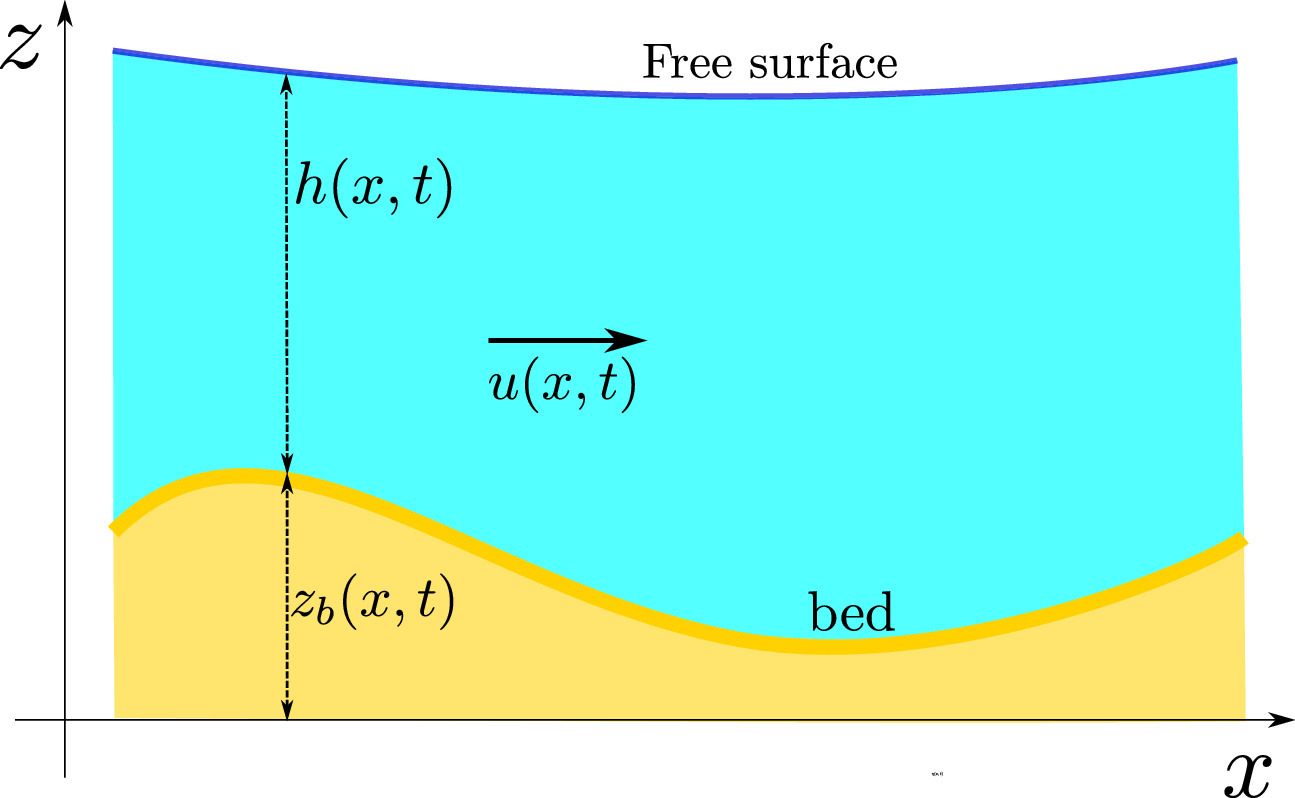
\includegraphics[width=10cm,height=6cm,keepaspectratio]{.//Pics//exner.jpg}
    \caption{Ecuación de Exner: evolución del lecho.}
    \end{figure}
\end{frame}

\begin{frame}{Ecuación de Exner}
    \begin{align}
    {\partial z_b \over \partial t} + \frac{1}{1-\lambda_p} \nabla\cdot \mathbf{q_s} = E-D,
    \end{align}
    donde $q_s$ es el flujo sólido superficial $(m^2/s)$ y $E, D (m/s)$ son erosión y deposición. Para un modelo reducido, se puede usar:
    \begin{align}
        \mathbf{q_s}=\gamma_shC\mathbf{u}
    \end{align}
    y un cierre simple para erosión/deposición (prototipo):
    \begin{align}
        E-D=\beta_e\|\mathbf{u}\|-\beta_dC,
    \end{align}
    con $\beta_e,\beta_d$ ajustables. En escenarios iniciales, muchas veces se fija $E-D = 0$ para congelar el lecho y validar primero la dinámica; 
    luego se activa Exner.
\end{frame}

%/////////////////////////////////////////////%
\section{Carta Gantt}
\begin{frame}{Carta Gantt I}
    \begin{table}
        \centering
        \caption{Planificación de Actividades (Marzo - Noviembre 2026)}
        \label{tab:planificacion_gantt1}
        \resizebox{\textwidth}{!}{%
        \begin{tabular}{|c|p{7cm}|c|c|c|} 
        \hline
        \textbf{ID} & \textbf{Actividad} & \textbf{Inicio} & \textbf{Término} & \textbf{Obj.} \\ \hline
        1 & Revisión bibliográfica de PINNs & 02/03/26 & 31/03/26 & OE1 \\ \hline
        2 & Definición de sistema de PDEs & 01/04/26 & 30/04/26 & OE1 \\ \hline
        3 & Programación de PINNs en Python & 04/05/26 & 22/05/26 & OE2 \\ \hline
        4 & Implementación de restricciones fuertes & 25/05/26 & 12/06/26 & OE2 \\ \hline
        5 & Obtención de predicciones adecuadas & 15/06/26 & 03/07/26 & OE2 \\ \hline
        6 & Config. de normalización y detenciones & 06/07/26 & 31/07/26 & OE3 \\ \hline
        7 & Redacción de Capítulos 1 y 2 & 03/08/26 & 21/08/26 & Doc. \\ \hline
        8 & Ajuste de IC/BC y masa inicial & 24/08/26 & 11/09/26 & OE3 \\ \hline
        9 & Entrenamiento de masa y momento & 14/09/26 & 09/10/26 & OE3 \\ \hline
        10 & Acople de concentración y presión & 12/10/26 & 06/11/26 & OE3 \\ \hline
        \end{tabular}%
        }
    \end{table}
\end{frame}

\begin{frame}{Carta Gantt II}
    \begin{table}
        \centering
        \caption{Planificación de Actividades (Noviembre 2026 - Marzo 2027)}
        \label{tab:planificacion_gantt2}
        
        \resizebox{\textwidth}{!}{%
        \begin{tabular}{|c|p{7cm}|c|c|c|}
        \hline
        \textbf{ID} & \textbf{Actividad} & \textbf{Inicio} & \textbf{Término} & \textbf{Obj.} \\ \hline
        11 & Técnicas para colapso a la trivialidad & 09/11/26 & 27/11/26 & OE3 \\ \hline
        12 & Optimizador y tasa de aprendizaje & 30/11/26 & 24/12/26 & OE3 \\ \hline
        13 & Redacción de capítulo 3 & 28/12/26 & 15/01/27 & Doc. \\ \hline
        14 & Sensibilidad y cuantif. de errores & 18/01/27 & 05/02/27 & OE3 \\ \hline
        15 & Validación vs Modelos numéricos & 08/02/27 & 26/02/27 & OE3 \\ \hline
        16 & Análisis y visualizaciones & 01/03/27 & 12/03/27 & OE4 \\ \hline
        17 & Redacción de capítulos 4 y 5 & 15/03/27 & 24/03/27 & Doc. \\ \hline
        18 & Revisión final, citas y bibliografía & 25/03/27 & 29/03/27 & Doc. \\ \hline
        19 & Preparación de defensa de tesis & 30/03/27 & 30/03/27 & Ex. \\ \hline
        20 & Entrega final y cierre & 31/03/27 & 31/03/27 & Hito \\ \hline
        \end{tabular}%
        }
    \end{table}
\end{frame}

\begin{frame}{Carta Gantt III}
    \begin{figure}[h!]
        \centering
        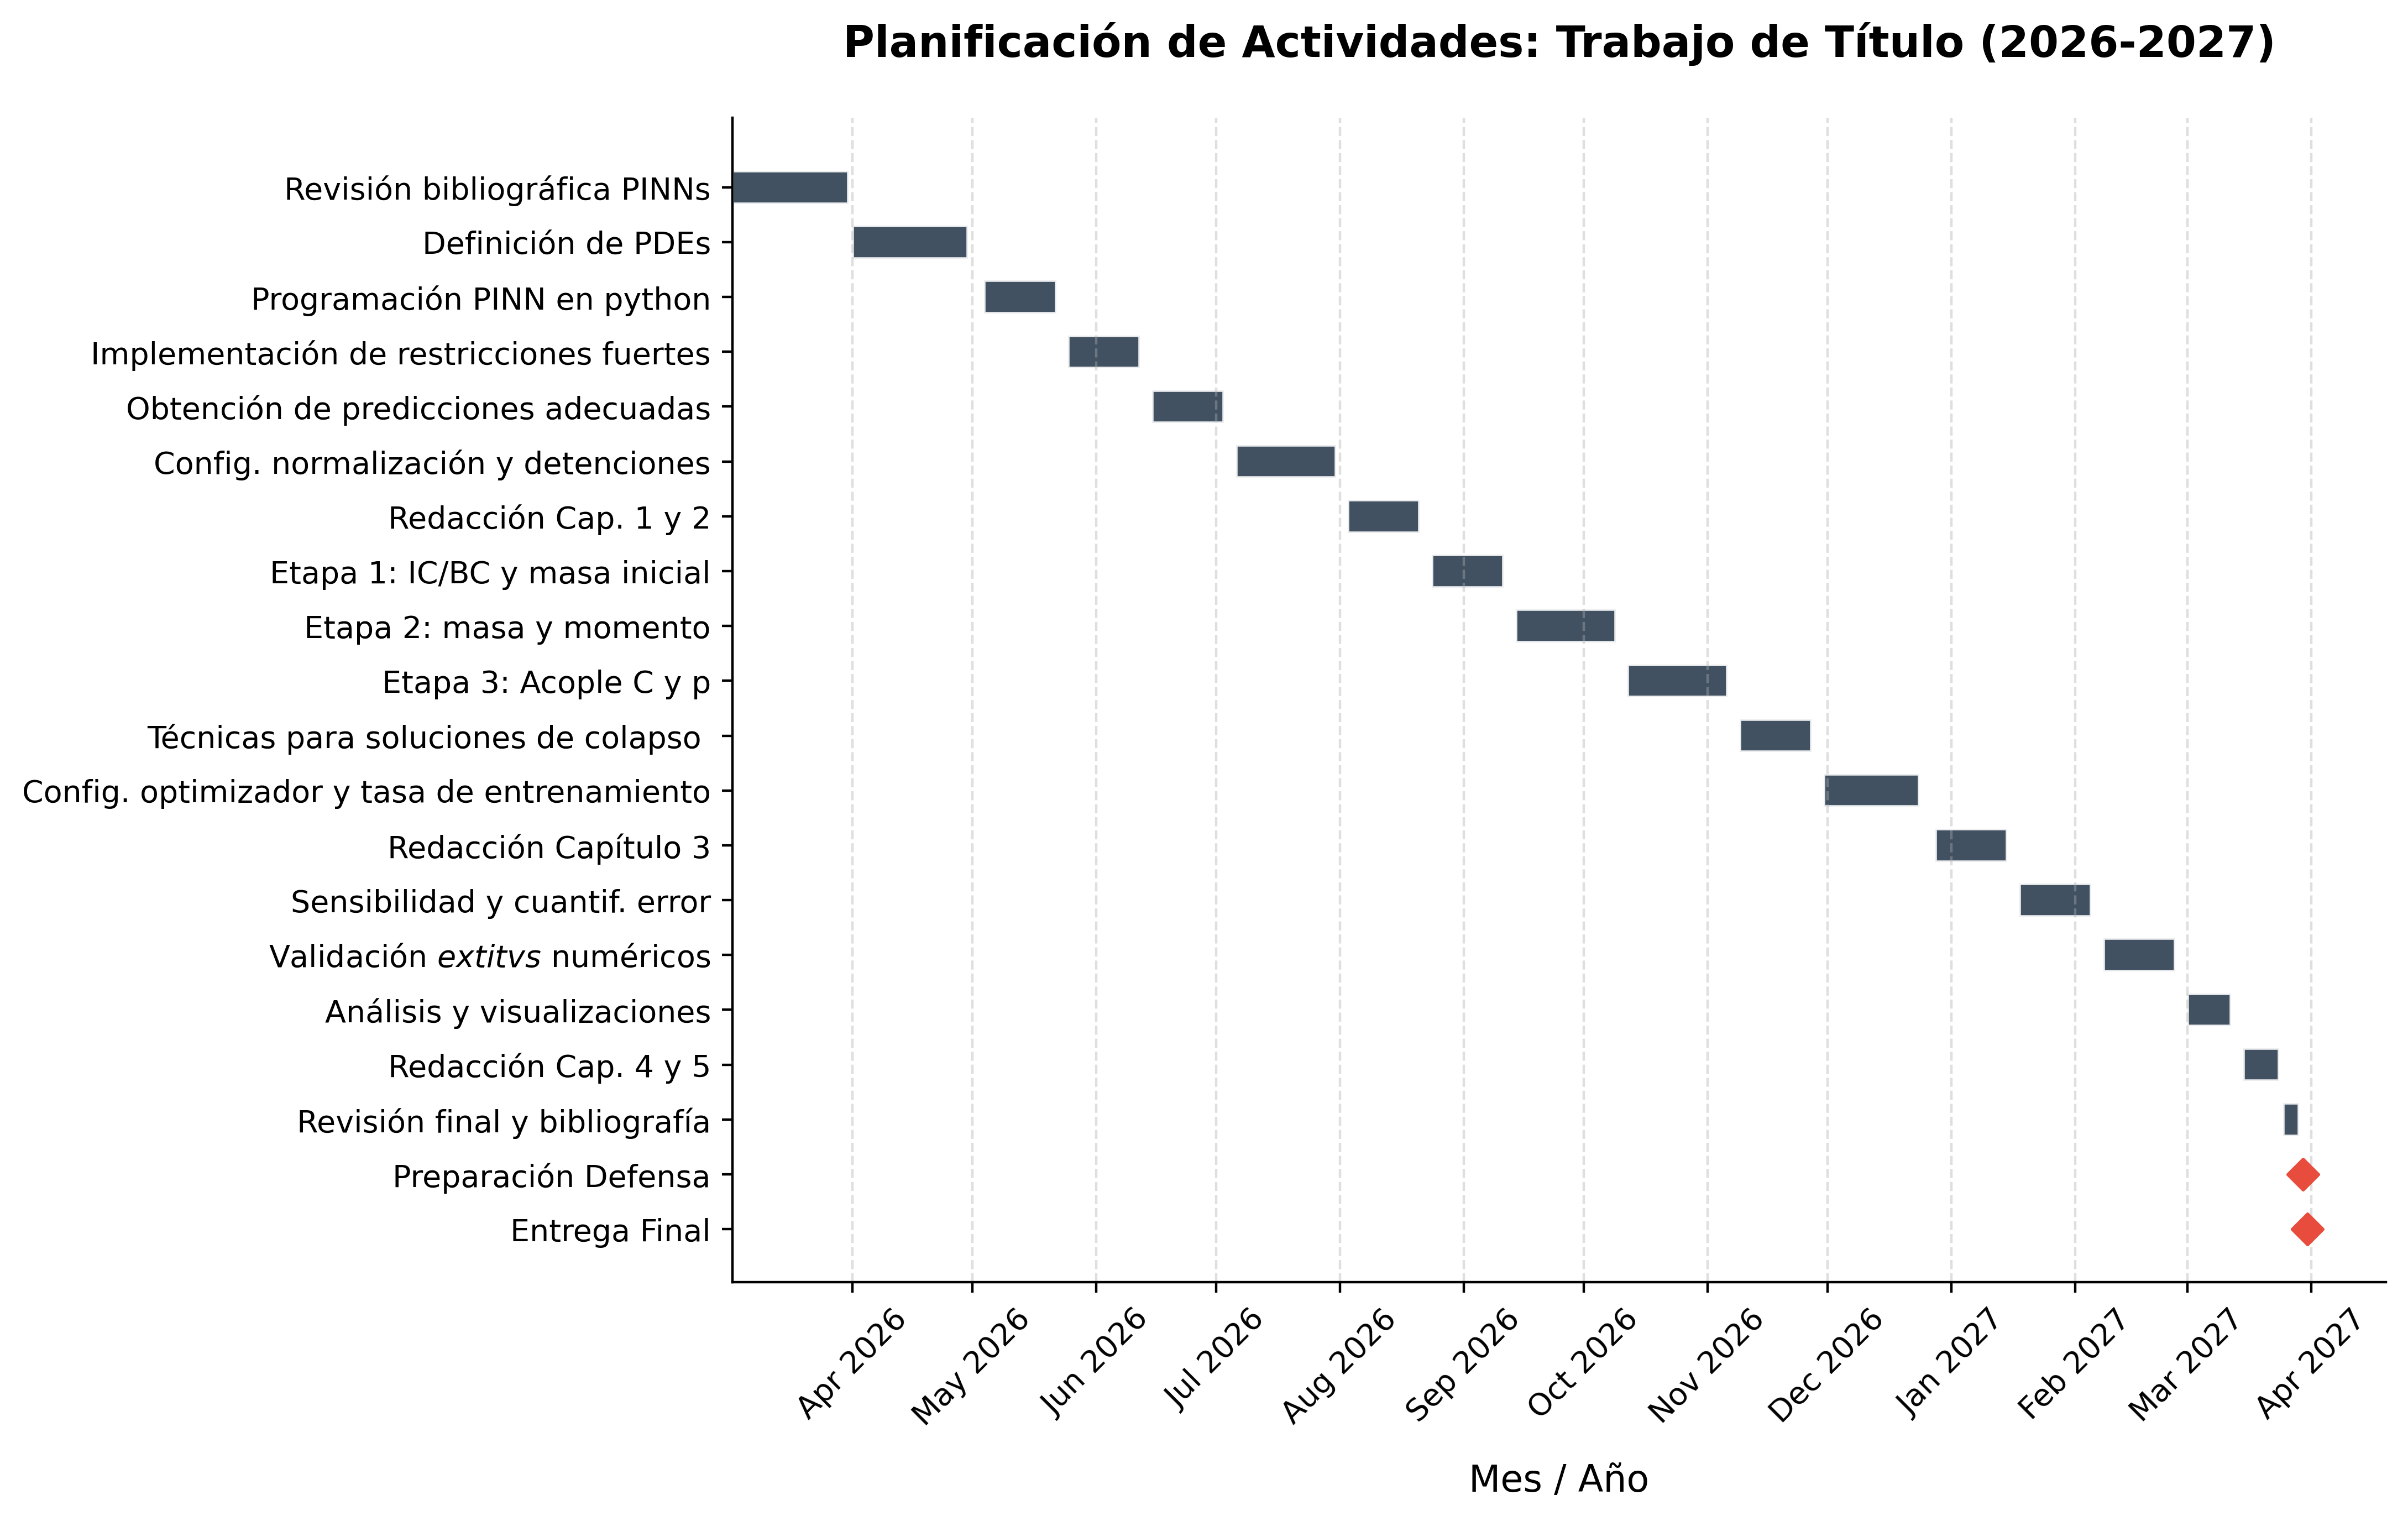
\includegraphics[width=\linewidth]{Pics/carta_gantt_formal.png}
        \caption{Carta Gantt de actividades para el desarrollo del trabajo de título.}
        \label{fig:gantt}
    \end{figure}
\end{frame}
%/////////////////////////////////////////////%
\section{Conclusiones} 
\begin{frame}{Conclusiones}
    \begin{enumerate}
        \item Se ha formulado un sistema acoplado de PDEs que modela la morfodinámica de un lahar, incorporando conservación de masa, momento, concentración sólida y presión de poros.
        \item El agregar más ecuaciones diferenciales parciales y parámetros geológicos al modelo de PINN permite capturar fenómenos físicos más complejos, pero también introduce desafíos significativos en términos de convergencia y estabilidad del entrenamiento.
    \end{enumerate}
\end{frame}



%/////////////////////////////////////////////%
\begin{frame}[allowframebreaks]{Referencias}
    \tiny
    % Esto cambia el ícono de documento por los números [1], [2] del estilo IEEE
    \setbeamertemplate{bibliography item}[text] 
    
    \nocite{*} % Muestra todas las referencias de tu archivo BibTesis.bib
    \bibliographystyle{ieeetr}
    \bibliography{BibTesis} % Asegúrate de que tu archivo se llame BibTesis.bib
\end{frame}

\end{document}